\documentclass[10pt,a4paper]{article}
\usepackage[T1]{fontenc}
\usepackage[utf8]{inputenc}
\usepackage[dutch]{babel}
\usepackage[margin=20mm,top=18mm,bottom=18mm,headheight=18pt,headsep=5mm]{geometry}
\usepackage{amsmath,amssymb}
\usepackage{graphicx}
\usepackage{booktabs}
\usepackage{xcolor}
\usepackage{fancyhdr}
\usepackage[font=small,labelfont=bf,skip=3pt]{caption}
\usepackage{enumitem}
\providecommand{\num}[1]{#1}
\setlist{itemsep=1pt,topsep=3pt,parsep=0pt}
\setlength{\parskip}{4pt}
\setlength{\parindent}{0pt}
\definecolor{qdat}{HTML}{1a1a1a}
\definecolor{han}{HTML}{E6006E}

% automatisch gegenereerd door analyse.py -- niet met de hand aanpassen
\newcommand{\RbMinPack}{73{,}2}
\newcommand{\RgapOpt}{24{,}8}
\newcommand{\RframeWOpt}{76{,}0}
\newcommand{\RbfWheel}{70{,}0}
\newcommand{\RclearTyre}{1{,}05}
\newcommand{\RtotalWOpt}{123{,}9}
\newcommand{\RWuOpt}{64}
\newcommand{\Rmtot}{0{,}539}
\newcommand{\Rmtotg}{539}
\newcommand{\RWn}{5{,}29}
\newcommand{\Rxg}{21{,}8}
\newcommand{\Rhcg}{46{,}4}
\newcommand{\RsigmaOpt}{70{,}9}
\newcommand{\RsigLo}{65}
\newcommand{\RsigHi}{80}
\newcommand{\RNdrive}{3{,}75}
\newcommand{\RNcaster}{1{,}54}
\newcommand{\RsensOpt}{1{,}33}
\newcommand{\RdSens}{67}
\newcommand{\RdLoSigma}{62{,}3}
\newcommand{\RdHiSigma}{109{,}0}
\newcommand{\RaLift}{4{,}60}
\newcommand{\RaLiftG}{0{,}47}
\newcommand{\RxgMin}{18{,}6}
\newcommand{\RaAccel}{3{,}72}
\newcommand{\RaAccelG}{0{,}38}
\newcommand{\RbRoll}{74{,}3}
\newcommand{\RaRoll}{10{,}35}
\newcommand{\RaSlip}{7{,}85}
\newcommand{\RdiagOpt}{29{,}1}
\newcommand{\RaDiag}{6{,}15}
\newcommand{\RTcaster}{23{,}0}
\newcommand{\RdsAxle}{10{,}05}
\newcommand{\RdsShaft}{0{,}209}
\newcommand{\RquantOpt}{5{,}88}
\newcommand{\RquantMin}{7{,}87}
\newcommand{\RquantShaft}{0{,}122}
\newcommand{\RcalOpt}{1{,}38}
\newcommand{\RcalMin}{1{,}84}
\newcommand{\RdriftOpt}{51}
\newcommand{\RdriftMin}{68}
\newcommand{\RquantGain}{25}
\newcommand{\RFstallEen}{1{,}55}
\newcommand{\RFstallTwee}{3{,}10}
\newcommand{\RFtracTwee}{3{,}00}
\newcommand{\RFtracVier}{4{,}23}
\newcommand{\RtracGain}{41}
\newcommand{\RFreqNul}{0{,}43}
\newcommand{\RFreqTien}{1{,}34}
\newcommand{\RmarginNul}{7{,}0}
\newcommand{\RmarginTien}{2{,}2}
\newcommand{\RgradeMaxTwee}{29}
\newcommand{\RgradeMaxVier}{40}
\newcommand{\Rvmax}{0{,}67}
\newcommand{\Rvwork}{0{,}38}
\newcommand{\RTyawTwee}{147}
\newcommand{\RTresTwee}{23{,}0}
\newcommand{\RTyawVier}{207}
\newcommand{\RTresVier}{106}
\newcommand{\RscrubTwee}{16}
\newcommand{\RscrubVier}{51}
\newcommand{\RLwb}{100}
\newcommand{\RIstallTwee}{1{,}6}
\newcommand{\RIstallVier}{3{,}1}
\newcommand{\RIchanVier}{1{,}6}
\newcommand{\RPdissVier}{4{,}2}
\newcommand{\RbAgile}{159}
\newcommand{\RalphaOpt}{140}
\newcommand{\RalphaMin}{119}
\newcommand{\RalphaGain}{18}
\newcommand{\RRswept}{90{,}0}
\newcommand{\RDswept}{180{,}0}
\newcommand{\RDsweptSquare}{195{,}4}
\newcommand{\RdMaxFoot}{85}
\newcommand{\RbAccu}{133{,}2}
\newcommand{\RbArea}{98}
\newcommand{\RAframe}{109{,}4}
\newcommand{\RAframeSmal}{133{,}1}
\newcommand{\RbSmalMin}{98}
\newcommand{\RAframeBreed}{140{,}4}
\newcommand{\RAframeGain}{28}
\newcommand{\RbSweptMax}{154}
\newcommand{\RxfOpt}{54}
\newcommand{\RxfSmal}{nan}
\newcommand{\RIfree}{0{,}12}
\newcommand{\RUpack}{6{,}0}
\newcommand{\RUm}{4{,}25}
\newcommand{\RVdrop}{1{,}38}
\newcommand{\RRpack}{0{,}60}
\newcommand{\RtauStallZes}{70}
\newcommand{\RIstallZes}{1{,}10}
\newcommand{\RnNulZes}{200}
\newcommand{\RUbat}{6}
\newcommand{\RomegaNul}{14{,}8}
\newcommand{\RtauCont}{14{,}0}
\newcommand{\RomegaCont}{10{,}7}
\newcommand{\RnCont}{102}
\newcommand{\RvCont}{0{,}34}
\newcommand{\RIcontEen}{0{,}31}
\newcommand{\RetaCont}{11}
\newcommand{\RPmechCont}{0{,}30}
\newcommand{\RPelekCont}{2{,}60}
\newcommand{\RUmMos}{5{,}00}
\newcommand{\RvMos}{0{,}41}
\newcommand{\RkDuty}{28{,}2}
\newcommand{\RFcont}{0{,}87}
\newcommand{\RmMaxVlak}{1100}
\newcommand{\RmMaxSnel}{675}
\newcommand{\RmMaxVijf}{603}
\newcommand{\RmMaxTien}{381}
\newcommand{\RmAdvies}{603}
\newcommand{\RmComp}{409}
\newcommand{\RmFrameNu}{130}
\newcommand{\RmRuimte}{64}
\newcommand{\RmFrameMax}{194}
\newcommand{\RIcont}{0{,}32}
\newcommand{\RaNu}{1{,}33}
\newcommand{\RmMosVijf}{669}
\newcommand{\RmMosWinst}{11}
\newcommand{\RzAxle}{32}
\newcommand{\RzMotLo}{21}
\newcommand{\RzMotHi}{43}
\newcommand{\RzDeckEen}{46}
\newcommand{\RzDeckTwee}{66}
\newcommand{\RzAccuLo}{46}
\newcommand{\RzTop}{93}
\newcommand{\RhStandoff}{17}
\newcommand{\RhLTweeNegenAcht}{27}
\newcommand{\RzTyre}{64}
\newcommand{\RhMaxPitch}{54{,}5}
\newcommand{\RhMaxRoll}{61{,}2}
\newcommand{\RhMax}{54{,}5}
\newcommand{\RmTopMax}{129}
\newcommand{\RhMarge}{8{,}0}
\newcommand{\RRfloor}{441}
\newcommand{\RzSRvier}{58}
\newcommand{\RzLijn}{8}
\newcommand{\RclearGround}{21}
\newcommand{\Rbreakover}{58}
\newcommand{\Rxmotf}{18}
\newcommand{\RaccuW}{58}
\newcommand{\RaccuL}{61}
\newcommand{\Rclear}{4}
\newcommand{\Rxrear}{90}
\newcommand{\RquantBreed}{3{,}79}
\newcommand{\RquantWinst}{36}
\newcommand{\RbOpt}{98}
\newcommand{\RdOpt}{75}
\newcommand{\Rrw}{32}
\newcommand{\RDw}{64}
\newcommand{\Rwtyre}{25{,}9}
\newcommand{\Rtgb}{22{,}6}
\newcommand{\Rewheel}{14}
\newcommand{\RLmot}{70}
\newcommand{\Rhmot}{22}
\newcommand{\Rmu}{0{,}80}
\newcommand{\Rmuc}{0{,}20}
\newcommand{\RLframe}{160}
\newcommand{\Repsb}{1{,}5}
\newcommand{\Rxmotr}{52}
\newcommand{\Rcrr}{0{,}03}
\newcommand{\REd}{1}
\newcommand{\RNaxle}{20}
\newcommand{\RNshaft}{960}
\newcommand{\Rtaustall}{50}
\newcommand{\RIstallEen}{0{,}8}
\newcommand{\RholeX}{30}
\newcommand{\RholeY}{25}


\pagestyle{fancy}
\fancyhf{}
\renewcommand{\headrulewidth}{0.4pt}
\fancyhead[L]{\footnotesize Optimale spoorbreedte, massalimiet en bouwhoogte}
\fancyhead[R]{\raisebox{-1.1mm}{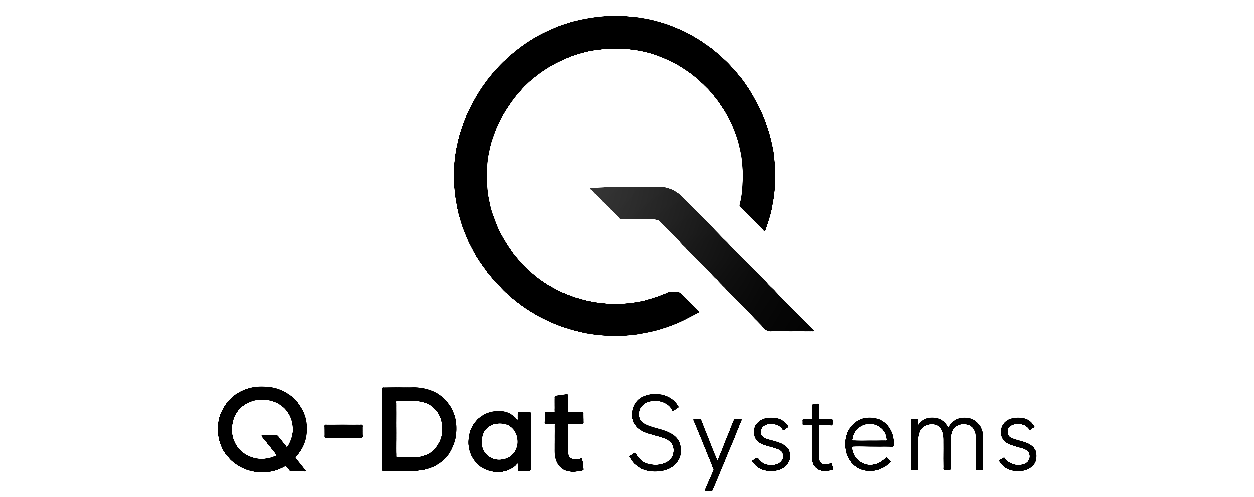
\includegraphics[height=4.5mm]{logo-qdat.png}}}
\fancyfoot[C]{\footnotesize\thepage}

\begin{document}
\thispagestyle{plain}
\noindent
\begin{minipage}[b]{0.5\textwidth}%
  
\includegraphics[height=15mm]{logo-han.png}%
\end{minipage}%
\begin{minipage}[b]{0.5\textwidth}%
  \raggedleft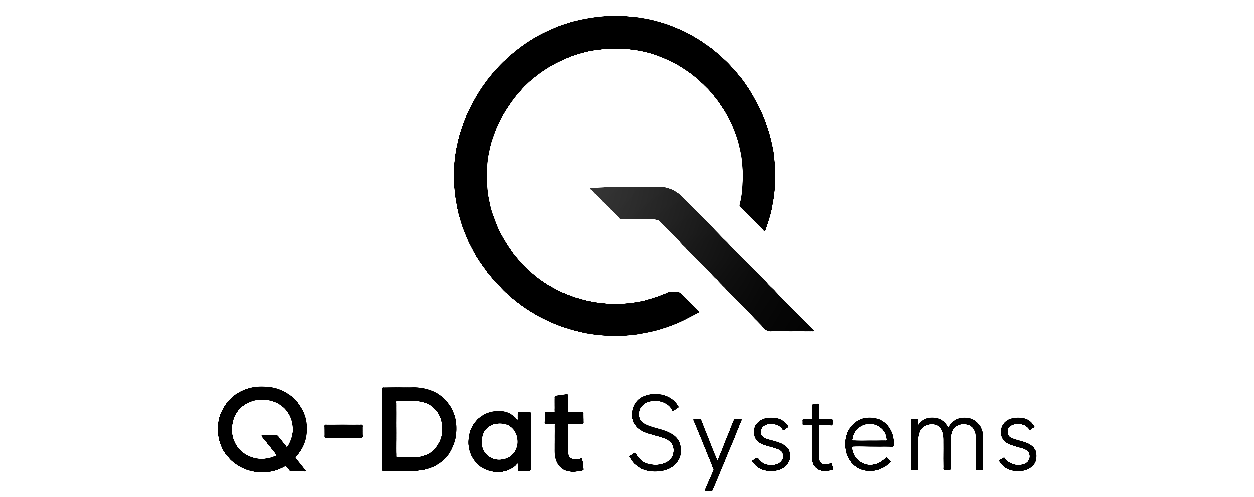
\includegraphics[height=11mm]{logo-qdat.png}%
\end{minipage}

\vspace{3mm}\hrule\vspace{6mm}

{\LARGE\bfseries Optimale spoorbreedte, massalimiet en bouwhoogte}\\[2mm]
{\large Custom frame voor een differentieel aangedreven autonome robotauto}\\[3mm]
{\small Q-Dat Systems \quad$\cdot$\quad Project 1 Embedded Systems \quad$\cdot$\quad \today\\[1mm]
Opgesteld door \textbf{Claude Opus 5} in opdracht van Tygo Poodt, op basis van de 1:1
CAD-modellen van de componenten en de databladen van motor en driver.}

\vspace{3mm}\hrule\vspace{4mm}

\textbf{\large Onderzoeksvragen}
\begin{enumerate}[label=\textbf{\arabic*.},leftmargin=8mm]
\item Welke spoorbreedte $b$ is optimaal voor een zelf te ontwerpen frame?
\item Hoe zwaar mag de auto worden met de twee gegeven motoren?
\item Op welke hoogte komen de componenten, en hoe hoog mag het zwaartepunt worden?
\end{enumerate}

\vspace{2mm}
\fbox{\parbox{\dimexpr\textwidth-2\fboxsep-2\fboxrule}{%
\textbf{Conclusie.}\quad
\textbf{(1)} $b = \RbOpt$~mm, hart band tot hart band. De platte 4$\times$AA-houder past niet
tussen de motoren, dus staat alles achter elkaar op twee dekken en is de smalste uitvoering de
zuinigste; \RbOpt~mm is het smalst waarop de Xplained Mini nog op een dek past.\quad
\textbf{(2)} $m \le \RmAdvies$~g totaal. Van de \RUpack~V uit vier AA-cellen komt maar
\RUm~V aan de motor; het werkpunt van het beste rendement ligt op $u^* = \RkDuty$~\% van het
blokkeerkoppel. Het ontwerp weegt \Rmtotg~g, dus er is nog maar \RmRuimte~g over.\quad
\textbf{(3)} Hoofddek op \RzDeckEen~mm, bovendek op \RzDeckTwee~mm, totale hoogte
\RzTop~mm. Het zwaartepunt moet onder \RhMax~mm blijven; het zit nu op \Rhcg~mm, goed voor
nog \RmTopMax~g extra op het bovendek.
}}

\section{Meetgegevens}

\begin{minipage}[t]{0.48\textwidth}
\footnotesize
\begin{tabular}{@{}llr@{}}
\multicolumn{3}{@{}l}{\textbf{Uit de 1:1 CAD-modellen}}\\
\toprule
$D$ & wieldiameter & \RDw~mm \\
$w$ & bandbreedte & \Rwtyre~mm \\
$t$ & dikte tandwielkast & \Rtgb~mm \\
$e$ & hart band buiten de kastwand & \Rewheel~mm \\
$L_m$ & motorlengte & \RLmot~mm \\
 & Xplained Mini & 60$\times$75~mm \\
 & breadboard half-size & 55$\times$84~mm \\
 & L298N-module & 43$\times$43~mm \\
 & accu 4$\times$AA, plat & 58$\times$61~mm \\
\bottomrule
\end{tabular}
\end{minipage}\hfill
\begin{minipage}[t]{0.48\textwidth}
\footnotesize
\begin{tabular}{@{}llr@{}}
\multicolumn{3}{@{}l}{\textbf{Uit de databladen en aannames}}\\
\toprule
$\tau_s$ & blokkeerkoppel bij \RUbat~V & \RtauStallZes~mNm \\
$I_s$ & blokkeerstroom bij \RUbat~V & \RIstallZes~A \\
$I_0$ & onbelaste stroom & \RIfree~A \\
$n_0$ & onbelast toerental bij \RUbat~V & \RnNulZes~rpm \\
$U_{\text{pak}}$ & 4$\times$AA alkaline & \RUpack~V \\
$R_{\text{pak}}$ & inwendige weerstand & \RRpack~$\Omega$ \\
$\mu$ & wrijving band -- vloer & \Rmu \\
$C_{rr}$ & rolweerstand & \Rcrr \\
$N$ & encoderpulsen per wielomw. & \RNaxle \\
$\epsilon_b$ & tolerantie spoorbreedte & \Repsb~mm \\
$E_d$ & wieldiameterverschil L/R & \REd~\% \\
\bottomrule
\end{tabular}
\end{minipage}

\vspace{2mm}
De kinematica van een differentieelaandrijving legt vast waarom juist $b$ telt:
\begin{equation}
\Delta s = \tfrac{1}{2}(s_R + s_L), \qquad \Delta\theta = \frac{s_R - s_L}{b}
\label{eq:kin}
\end{equation}
Dit is exact zolang de wielen zuiver rollen. De motorafstand $g$ (vrije ruimte tussen de
tandwielkasten) vertaalt naar $b$ via
\begin{equation}
b = g + 2(t+e) = g + \RbMinPack~\text{mm},\qquad
B_{\text{frame}} = g + 2t,\qquad B_{\text{buiten}} = b + w
\label{eq:pak}
\end{equation}

\begin{figure}[htbp]
\centering
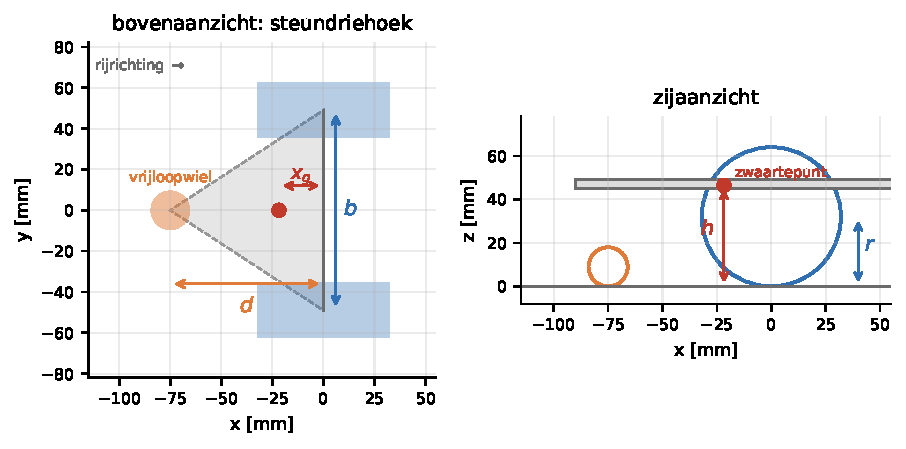
\includegraphics[width=0.86\textwidth]{figuren/f1_definities.pdf}
\caption{Symbolen. Oorsprong midden op de aandrijfas, vloerniveau, $x$ naar voren.}
\end{figure}

\section{Vraag 1: de optimale spoorbreedte}

\subsection{Wat breder maken oplevert}
Alle odometriefouten schalen met $1/b$: de hoekstap per encoderpuls, de fout door een
tolerantie $\epsilon_b$ in de effectieve spoorbreedte, en de koersdrift door een
diameterverschil $E_d$ over een afstand $L$:
\begin{equation}
\delta\theta = \frac{\pi D}{N b},\qquad
\frac{\Delta\theta}{\theta} = \frac{\epsilon_b}{b},\qquad
y(L) = \frac{L^2 E_d}{2b}
\label{eq:odo}
\end{equation}
Bij $b = \RbOpt$~mm geeft dat \RquantOpt$^\circ$ per puls, \RcalOpt$^\circ$ na een bocht van
$90^\circ$ en \RdriftOpt~mm drift per meter. Zijdelings kantelen speelt niet: de auto glijdt
eerder weg dan dat hij kiepert zodra $b \ge 2\mu h = \RbRoll$~mm.

\emph{Belangrijker dan de breedte:} met de sleufschijf op de motoras in plaats van op de
wielas gaat $\delta\theta$ van \RquantOpt$^\circ$ naar \RquantShaft$^\circ$, een factor 48.
Daarmee vervalt het sterkste argument om breder te bouwen dan strikt nodig.

\subsection{Wat breder maken kost}
Voor elke $b$ is de bruikbare dekbreedte bepaald en is met een plankjes-indeling
(90$^\circ$ draaien toegestaan, \Rclear~mm speling) de kortste framelengte gezocht waarop de
vier componenten op \emph{twee} dekken passen. Drie dekken telt niet: dat tilt $h$ op en
vreet de kantelmarge uit~\eqref{eq:stat} op. Het frame-oppervlak $A(b) = L(b)\cdot
B_{\text{frame}}(b)$ heeft daardoor een minimum:
\begin{equation}
A(\RbArea) = \RAframe~\text{cm}^2
\quad\text{tegen}\quad
\RAframeSmal~\text{cm}^2 \text{ smaller en } \RAframeBreed~\text{cm}^2 \text{ bij } 152~\text{mm}
\label{eq:area}
\end{equation}
De platte 4$\times$AA-houder is \RaccuW~mm breed en past pas tussen de motoren vanaf
$b = \RbAccu$~mm --- veel te breed. Hij gaat dus hoe dan ook op een dek, en dan past er niets
meer naast elkaar: met een bruikbare dekbreedte van \RWuOpt~mm staat alles achter elkaar en ligt
de framelengte vast op \RxfOpt~mm vóór plus \Rxrear~mm achter de as. Het oppervlak
$A = L\cdot B_{\text{frame}}$ is dan alleen nog evenredig met de breedte, dus wint de smalste
uitvoering --- en die wordt begrensd door de Xplained Mini: die is 60~mm breed en past pas op
een dek vanaf $b = \RbArea$~mm. Breder maken kost recht evenredig meer frame
(\RAframeGain~\% bij 152~mm) voor \RquantWinst~\% betere hoekresolutie: een slechte ruil. De
draaicirkel blijft tot $b = \RbSweptMax$~mm gewoon $\varnothing\,\RDswept$~mm.

\begin{figure}[htbp]
\centering
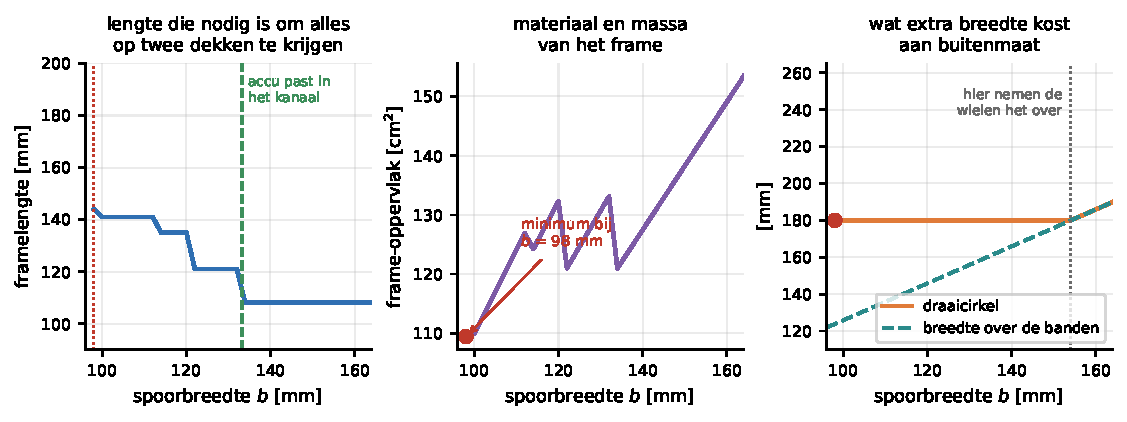
\includegraphics[width=0.96\textwidth]{figuren/f7_breedte.pdf}
\caption{Links: onder \RbAccu~mm groeit het frame in de lengte. Midden: daardoor een minimum
in het oppervlak bij \RbArea~mm. Rechts: breder maken kost tot \RbSweptMax~mm niets aan
draaicirkel, wel aan buitenmaat.}
\end{figure}

\begin{figure}[htbp]
\centering
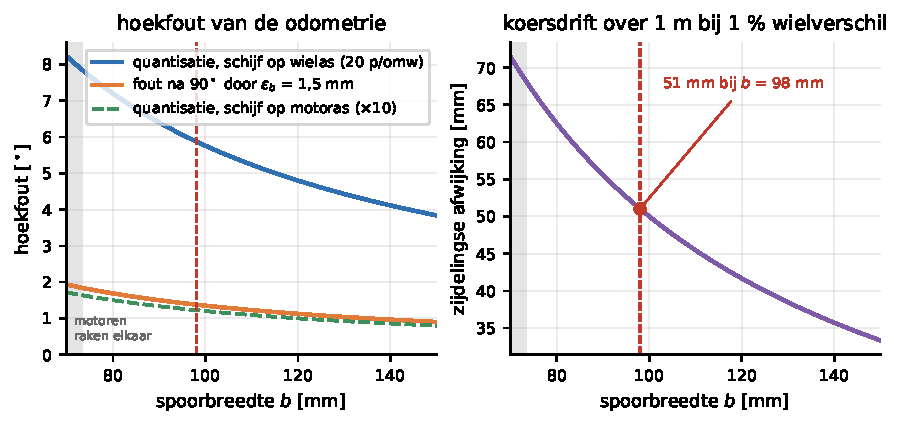
\includegraphics[width=0.96\textwidth]{figuren/f3_odometrie.pdf}
\caption{De drie foutbronnen uit~\eqref{eq:odo}, alle evenredig met $1/b$.}
\end{figure}

\section{Vraag 2: hoeveel massa mogen de motoren trekken}

\subsection{Motormodel}
De motor krijgt niet de pakspanning. De vier AA-cellen zakken in onder belasting en de
L298 slikt een vrijwel vaste verzadigingsval. Met twee motoren die elk $I$ trekken geldt
\begin{equation}
U_m = U_{\text{pak}} - 2I\,R_{\text{pak}} - \bigl(V_{d0} + V_{d1}I\bigr)
\qquad\Longrightarrow\qquad U_m = \RUm~\text{V}
\label{eq:voeding}
\end{equation}
Van de \RUpack~V blijft dus \RUm~V over; de L298 alleen kost al \RVdrop~V. Omdat alle
motorconstanten lineair met de klemspanning schalen, is dit een vaste-puntiteratie: het
werkpunt bepaalt de stroom en de stroom bepaalt de spanning.

Een gelijkstroommotor met borstels bij klemspanning $U_m$ heeft een lineaire
koppel-toerentalkarakteristiek. Met $u = \tau/\tau_s$ als belastingsgraad aan de uitgaande as:
\begin{equation}
\tau(u) = u\,\tau_s, \qquad
\omega(u) = \omega_0\,(1-u), \qquad
I(u) = I_0 + (I_s - I_0)\,u
\label{eq:motor}
\end{equation}
Blokkeren ($u=1$) is geen werkpunt: alle elektrische energie wordt dan warmte. Het zinvolle
duurzame werkpunt is dat van het beste rendement, want dat levert het meeste nuttige werk per
ampère\-uur accu en produceert daarmee ook de minste warmte. Met
$\eta(u) = \tau\omega/(UI)$ geldt
\begin{equation}
\eta(u) = \frac{\tau_s\,\omega_0\;u(1-u)}{U\,\bigl(I_0 + (I_s-I_0)u\bigr)},
\qquad
\frac{\mathrm{d}\eta}{\mathrm{d}u} = 0
\;\Longrightarrow\;
(I_s-I_0)\,u^2 + 2I_0\,u - I_0 = 0
\label{eq:eta}
\end{equation}
De fysisch zinvolle wortel is
\begin{equation}
\boxed{\;u^* = \frac{\sqrt{I_0 I_s} - I_0}{I_s - I_0}\;}
\qquad\Rightarrow\qquad
u^* = \frac{\sqrt{\RIfree \cdot \RIstallEen} - \RIfree}{\RIstallEen - \RIfree} = \RkDuty~\%
\label{eq:ustar}
\end{equation}
Invullen in~\eqref{eq:motor}, met de constanten geschaald naar $U_m$, geeft het werkpunt per
motor: koppel \RtauCont~mNm, toerental \RnCont~rpm (dus $v = \omega r = \RvCont$~m/s),
stroom \RIcontEen~A, rendement \RetaCont~\% inclusief de tandwielkast. Voor twee motoren
samen is dat \RPmechCont~W nuttig uit \RPelekCont~W elektrisch.

\subsection{Massalimiet}
De duurzame trekkracht van twee motoren aan de wielomtrek is
\begin{equation}
F_c = \frac{2\,u^*\tau_s}{r} = \RFcont~\text{N}
\label{eq:Fc}
\end{equation}
De rijweerstand van een auto met massa $m$ op een helling $\theta$ bij versnelling $a$ is
$F = m\bigl(a + g(C_{rr}\cos\theta + \sin\theta)\bigr)$. Gelijkstellen geeft
\begin{equation}
\boxed{\;m_{\max}(a,\theta) = \frac{2\,u^*\tau_s / r}{a + g\,(C_{rr}\cos\theta + \sin\theta)}\;}
\label{eq:massa}
\end{equation}
Grip begrenst de massa niet: de eis $F \le \mu\sigma m g$ heeft $m$ aan beide kanten, want
zwaarder betekent evenveel méér grip. Alleen het koppel is bepalend.

\begin{center}
\footnotesize
\begin{tabular}{@{}llr@{}}
\toprule
Rijgeval & & $m_{\max}$ \\
\midrule
vlakke vloer, $a = 0{,}5$~m/s$^2$ & ruim & \RmMaxVlak~g \\
vlakke vloer, $a = 1{,}0$~m/s$^2$ & vlot optrekken & \RmMaxSnel~g \\
\textbf{drempel $5^\circ$, $a = 0{,}3$~m/s$^2$} & \textbf{maatgevend} & \textbf{\RmAdvies~g} \\
helling $10^\circ$, $a = 0{,}3$~m/s$^2$ & zwaar & \RmMaxTien~g \\
\bottomrule
\end{tabular}
\end{center}

Aanhouden: \textbf{\RmAdvies~g}. Het ontwerp weegt nu \Rmtotg~g (\RmComp~g componenten,
\RmFrameNu~g frame), dus er is nog maar \RmRuimte~g over en het frame mag hooguit
\RmFrameMax~g worden. Dat is krap: houd het printvolume laag en weeg de gebouwde auto na.
De stroom blijft \RIcontEen~A per motor, ruim binnen de 2~A per L298-kanaal.

\textbf{De grootste winst zit in de driver.} De L298 kost \RVdrop~V van de \RUpack~V, oftewel
een kwart van het beschikbare vermogen. Een MOSFET-driver (bijvoorbeeld TB6612FNG, samen zo'n
0,5~V val) brengt $U_m$ van \RUm~V naar \RUmMos~V: \RmMosWinst~\% meer trekkracht,
\RmMosVijf~g in plaats van \RmAdvies~g, en \RvMos~m/s in plaats van \RvCont~m/s. Dat is
goedkoper dan gewicht besparen.

\begin{figure}[htbp]
\centering
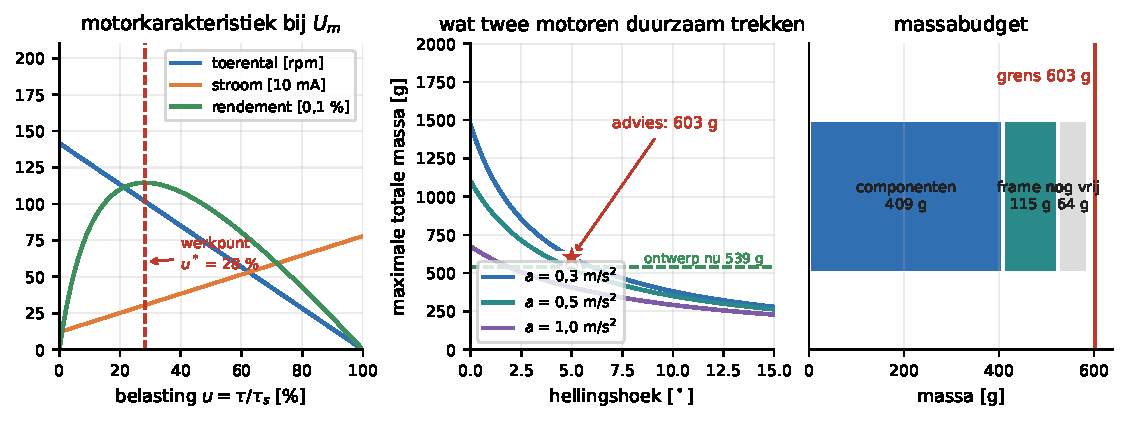
\includegraphics[width=0.96\textwidth]{figuren/f8_massa.pdf}
\caption{Links: de karakteristiek~\eqref{eq:motor} met het werkpunt uit~\eqref{eq:ustar}.
Midden: $m_{\max}$ volgens~\eqref{eq:massa}. Rechts: het massabudget.}
\end{figure}

\section{Vraag 3: op welke hoogte de componenten komen}

De verticale opbouw ligt grotendeels vast zodra de motor gekozen is. De aandrijfas zit op
$r = \Rrw$~mm; het motorhuis is \Rhmot~mm hoog en symmetrisch om die as, dus van
\RzMotLo~mm tot \RzMotHi~mm. Het hoofddek moet daaroverheen: met een plaat van 3~mm komt de
bovenkant op \RzDeckEen~mm. Het hoogste onderdeel daarop is de L298N met koellichaam
(\RhLTweeNegenAcht~mm), dus het bovendek komt op \RzDeckTwee~mm --- afstandbussen van
\RhStandoff~mm --- en de bovenkant van het breadboard op \RzTop~mm.

De enige echte vrijheid is hoe zwaar je bovenin bouwt, en die wordt begrensd door de
kantelmarge uit~\eqref{eq:stat}:
\begin{equation}
a_{\text{kantel}} = g\,\frac{x_g}{h} \ge 0{,}4\,g
\quad\Longrightarrow\quad
h \le \frac{x_g}{0{,}4} = \RhMaxPitch~\text{mm}
\qquad\text{(zijdelings: } h \le \tfrac{b}{2\mu} = \RhMaxRoll\text{ mm, ruimer)}
\label{eq:hoogte}
\end{equation}
Het ontwerp zit op $h = \Rhcg$~mm en heeft dus \RhMarge~mm marge. Vertaald naar massa mag er
nog \textbf{\RmTopMax~g} bij op het bovendek voordat $h$ de grens raakt. Dat is minder dan de
\RmRuimte~g die het motorbudget nog toelaat: \emph{boven het bovendek is de hoogte eerder op dan
het gewicht.} Zware uitbreidingen horen dus laag, bij voorkeur in het kanaal naast de accu.

Twee maten volgen nog uit de opbouw. De bodemvrijheid is \RclearGround~mm (de onderkant van de
accu is het laagste punt), goed voor een hellingdoorgang van \Rbreakover$^\circ$. En de
HC-SR04 op \RzSRvier~mm met een halve openingshoek $\beta = 7{,}5^\circ$ verlicht de vloer pas
vanaf $R = z/\tan\beta = \RRfloor$~mm; daarbuiten zijn vloerechos mogelijk. Monteer hem zo hoog
als de zwaartepunteis toelaat en kantel hem een paar graden omhoog.

\begin{figure}[htbp]
\centering
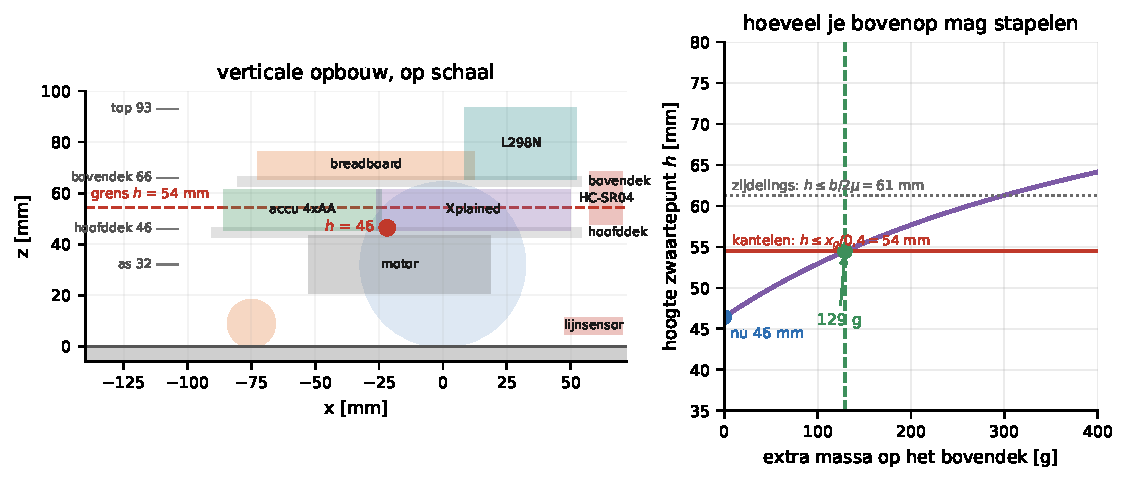
\includegraphics[width=0.98\textwidth]{figuren/f9_hoogte.pdf}
\caption{Links: de verticale opbouw op schaal. Rechts: het zwaartepunt loopt tegen de grens
uit~\eqref{eq:hoogte} aan bij \RmTopMax~g extra op het bovendek.}
\end{figure}

\section{Randvoorwaarden die hieruit volgen}

\subsection{Plaats van het vrijloopwiel}
Statisch evenwicht om de aandrijfas geeft het gewichtsaandeel $\sigma$ op de aandrijfwielen,
de gevoeligheid daarvan voor bouwtoleranties, en de vertraging waarbij het wieltje loskomt:
\begin{equation}
\sigma = 1 - \frac{x_g}{d},
\qquad
\frac{\partial\sigma}{\partial x_g} = -\frac{1}{d},
\qquad
a_{\text{kantel}} = g\,\frac{x_g}{h}
\label{eq:stat}
\end{equation}
$d$ valt uit $a_{\text{kantel}}$ weg: de kantelmarge hangt alleen van $x_g$ en $h$ af. Met
$x_g = \Rxg$~mm en $h = \Rhcg$~mm is die \RaLiftG~$g$, ruim boven de eis van 0,4~$g$. De
grenzen op $d$ komen dus uit de gevoeligheid ($\le$ 1,5 procentpunt per mm, dus
$d \ge \RdSens$~mm) en de draaicirkel ($\le$ 200~mm, dus $d \le \RdMaxFoot$~mm). Gekozen:
$d = \RdOpt$~mm, waarmee $\sigma = \RsigmaOpt$~\%.

\begin{figure}[htbp]
\centering
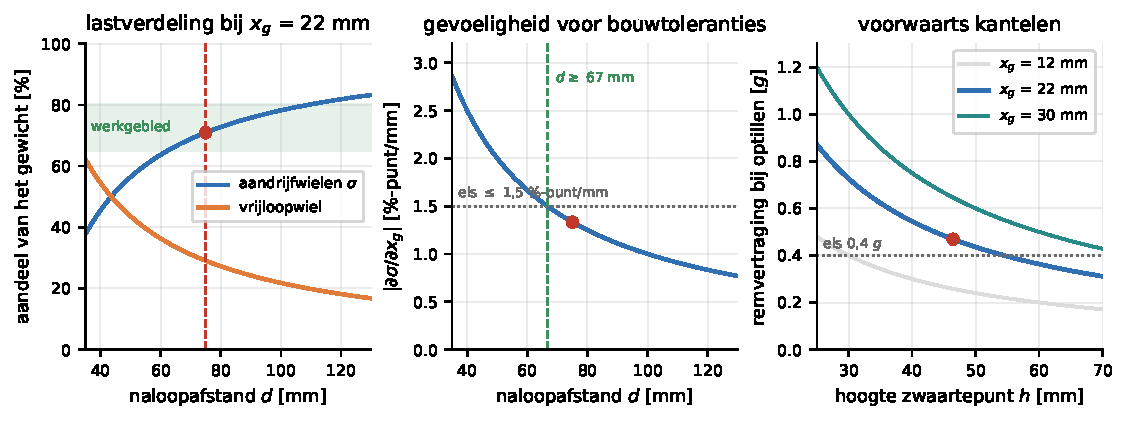
\includegraphics[width=0.96\textwidth]{figuren/f2_lastverdeling.pdf}
\caption{Lastverdeling, gevoeligheid en kantelmarge volgens~\eqref{eq:stat}.}
\end{figure}

\subsection{Twee motoren, geen vier}
\begin{center}
\footnotesize
\begin{tabular}{@{}lrr@{}}
\toprule
 & 2 aangedreven wielen & 4 aangedreven wielen \\
\midrule
grip $\mu\sigma mg$ resp. $\mu mg$ & \RFtracTwee~N & \RFtracVier~N \quad(+\RtracGain~\%) \\
blokkeerstroom per L298-kanaal & \RIstallEen~A & \RIchanVier~A \quad(limiet 2~A) \\
verlies aan schuifwrijving bij spinnen & \RscrubTwee~\% & \RscrubVier~\% \\
geldigheid van~\eqref{eq:kin} & exact & ondergrond- en snelheidsafhankelijk \\
\bottomrule
\end{tabular}
\end{center}
Nodig is \RFreqNul~N vlak en \RFreqTien~N op $10^\circ$; met twee wielen is \RFtracTwee~N
beschikbaar, marge \RmarginNul{} resp.\ \RmarginTien. De extra grip van vier motoren is dus
niet nodig, en kost de exactheid van~\eqref{eq:kin} --- voor een auto die op dead reckoning
vaart de duurste post.

\section{Bouwmaten}

\begin{minipage}[t]{0.44\textwidth}
\footnotesize\vspace{0pt}
\begin{tabular}{@{}llr@{}}
\toprule
$b$ & spoorbreedte & \textbf{\RbOpt~mm} \\
$m$ & maximale massa & \textbf{\RmAdvies~g} \\
\midrule
$g$ & ruimte tussen de kasten & \RgapOpt~mm \\
 & frame naast de banden & \RbfWheel~mm \\
 & frame ervoor en erachter & \RframeWOpt~mm \\
 & buitenmaat over de banden & \RtotalWOpt~mm \\
$d$ & naloopafstand & \RdOpt~mm \\
$x_g$ & zwaartepunt achter de as & \Rxg~mm \\
$h$ & hoogte zwaartepunt & $\le$ \Rhcg~mm \\
$\varnothing$ & draaicirkel & \RDswept~mm \\
$v$ & rijsnelheid in het werkpunt & \RvCont~m/s \\
\midrule
 & hoofddek (bovenkant) & \RzDeckEen~mm \\
 & bovendek (bovenkant) & \RzDeckTwee~mm \\
 & afstandbussen ertussen & \RhStandoff~mm \\
 & totale bouwhoogte & \RzTop~mm \\
 & bodemvrijheid & \RclearGround~mm \\
\bottomrule
\end{tabular}
\end{minipage}\hfill
\begin{minipage}[t]{0.53\textwidth}
\vspace{0pt}
\begin{enumerate}[leftmargin=5mm]
\item \textbf{Naast de banden mag het frame maar \RbfWheel~mm breed zijn}: tussen kastwand en
band zit \RclearTyre~mm. Ervoor en erachter mag \RframeWOpt~mm. Kost niets: het breedste
onderdeel is 60~mm en het bruikbare dek is \RWuOpt~mm.
\item \textbf{Meet $e$ na met de schuifmaat.} De \Rewheel~mm uit~\eqref{eq:pak} komt uit de
CAD; 2~mm fout verschuift $b$ met 4~mm.
\item \textbf{Sleufgaten} voor het vrijloopwiel, $\pm 8$~mm in de rijrichting. Patroon
\RholeX$\times$\RholeY~mm, de \RholeX{} in de lengte.
\item \textbf{Rond de achterkant af} langs de boog met straal $d+15$~mm: $\varnothing\,\RDswept$
in plaats van $\varnothing\,\RDsweptSquare$~mm.
\item \textbf{Accu laag en achter} in het kanaal van \RgapOpt~mm: drukt $h$ omlaag en $x_g$
omhoog, beide gunstig volgens~\eqref{eq:stat}.
\item \textbf{Encoderschijf op de motoras}, niet op de wielas.
\end{enumerate}
\end{minipage}

\begin{figure}[htbp]
\centering
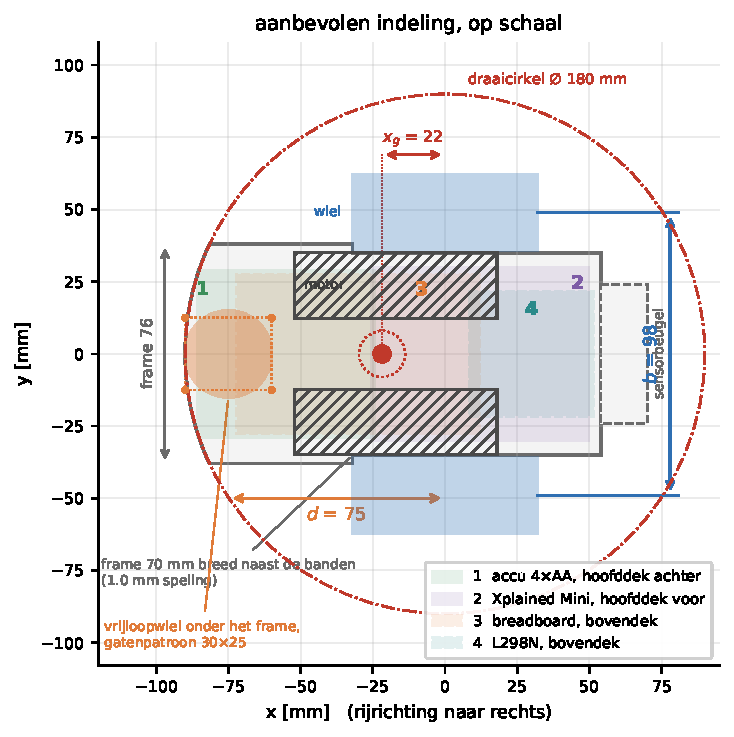
\includegraphics[width=0.66\textwidth]{figuren/f6_indeling.pdf}
\caption{Indeling op schaal, met de versmalling naar \RbfWheel~mm ter hoogte van de banden.}
\end{figure}

\vspace{1mm}\hrule\vspace{1mm}
{\footnotesize \textbf{Geldigheid.} Alle getallen komen uit \texttt{analyse.py} in dezelfde
map, dat ook de figuren en \texttt{resultaten.tex} genereert. Het blokkeerkoppel
\Rtaustall~mNm is een databladwaarde; opgaven voor deze motorklasse lopen van 35 tot 80~mNm en
$m_{\max}$ schaalt daar recht evenredig mee. De wrijvingscoëfficiënten gelden voor een gladde
vloer. De massalimiet is berekend voor een drempel van $5^\circ$; op een volledig vlakke baan
mag de auto tot \RmMaxVlak~g wegen.}

\end{document}
